
\begin{frame}{Reactive walking pattern generation \only<4>{with obstacles}}
\framesubtitle{\textcolor{green!30!black!80}{(M. Naveau, RA-L 2016)}}

  \begin{minipage}{0.48\textwidth}
  \vspace*{0.2cm}
    Optimization problem solved:
    \vspace*{-0.3cm}
    \only<1-3>{
        \begin{equation*}
          \begin{aligned}
            \min_{{\bf U}_k} 
            \sum_{i=0}^{j=4} w_i J_i({\bf U}_{k}) & \\
                {\bf X}_{k+1} = {\bf A}{\bf X}_{k} + {\bf C} {\bf U}_k & \\
                \underline{\bf P} < {\bf P} {\bf U}_k  < \overline{\bf P}& \\
          \end{aligned}
        \end{equation*}
        with ${\bf U}_k=\begin{pmatrix} \dddot{\bf X}_k \; {\bf X}_k^\mathit{f}\; \dddot{\bf Y}_k \;{\bf Y}_k^\mathit{f}  \end{pmatrix}^T$ \\        
      }
      \only<4>{
        \begin{equation*}
          \begin{aligned}
            \min_{{\bf U}_k} 
            \sum_{i=0}^{j=4} w_i J_i({\bf U}_{k}) & \\
                {\bf X}_{k+1} = {\bf A}{\bf X}_{k} + {\bf C} {\bf U}_k & \\
                \underline{\bf P} < {\bf P}{\color{red}{({\bf U}_k)}} {\bf U}_k  < \overline{\bf P}& \\
          \end{aligned}
        \end{equation*}
      with ${\bf U}_k=\begin{pmatrix} \dddot{\bf X}_k \; {\bf X}_k^\mathit{f}\; \dddot{\bf Y}_k \;{\bf Y}_k^\mathit{f} \;\color{red}{{\bf \Theta}_k^\mathit{f}}\end{pmatrix}^T$ \\
      }
  \end{minipage}
  %
  \begin{minipage}{0.48\textwidth}
    \only<1-3>{
      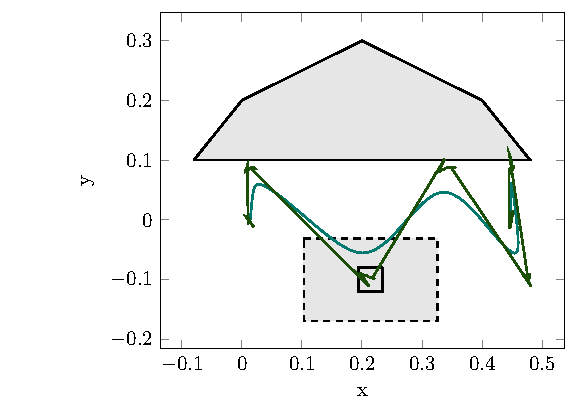
\includegraphics[width=\textwidth]{./images/tikz/convexHulls2}
    }
    \only<4>{
      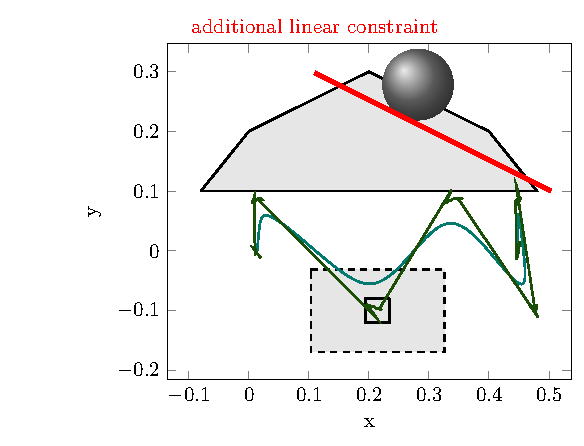
\includegraphics[width=\textwidth]{./images/tikz/convexHullsplusObstacles2}
    }
  \end{minipage}\\

  \only<1>{
    $J_1({\bf U}_{k})$ is the linear velocity tracking 
    {\small
      \begin{equation*}
        J_1({\bf U}_k) = \lVert \dot {\bf X}_{k} - {\bf X}_{k}^{ref} \rVert^2_2
        +  \lVert \dot {\bf Y}_{k} - {\bf Y}_{k}^{ref} \rVert^2_2 
      \end{equation*}}
    }
    \only<2>{$J_2({\bf U}_{k})$ is the control norm
      {\small
        \begin{equation*}
          J_2({\bf U}_k) = \lVert \dddot {\bf X}_{k} \rVert^2_2
          + \lVert \dddot {\bf Y}_{k} \rVert^2_2
        \end{equation*}
      }
    }
    \only<3>{$J_3({\bf U}_{k})$ is distance of the CoP to the most stable trajectory
      {\small
        \begin{equation*}
          J_3({\bf U}_k) = \lVert {\bf X}_{k}^{f} - CoP_{k+1}^{x} \rVert^2_2 +
          \lVert {\bf Y}_{k+1}^{f} - CoP_{k+1}^{y} \rVert^2_2 
        \end{equation*}
      }
    }
    \only<4>{$J_4({\bf U}_{k})$ is the angular velocity tracking
      {\small
        \begin{equation*}
            J_4({\bf U}_k) = \lVert {\bf \Theta}_{k} 
            - \int {\bf \Theta}_{k}^{ref} dt \; \rVert_2^2 
        \end{equation*}}
    }    

\end{frame}

%%%%%%%%%%%%%%%%%%%%%%%%%%%%%%%%%%%%%%%%%%%%%%%%%%%%%%%%%%%%%%%%%%%%%%%%%%%%%%%

\begin{frame}{Solver}
\begin{minipage}{0.48\textwidth}
Quadratic approximation :
\begin{equation*}
\begin{aligned}
    \min_{{\Delta \bf U}_k} \sum_{i=0}^{j=4} w_i 
    \left(
      J_i({\bf U}_{k-1}) +
      \nabla_{{\bf U}_k} J_i|_{{\bf U}_{k-1}}\,^T {\Delta \bf U}_k +
      {\Delta \bf U}_k^T \nabla ^{2}_{{\bf U}_k} J_i|_{{\bf U}_{k-1}}\,^T {\Delta \bf U}_k
    \right)\\
    {\bf U}_{k} = {\bf U}_{k-1} {\Delta \bf U}_k \\
    {\bf X}_{k+1} = {\bf A}{\bf X}_{k} + {\bf C} {\bf U}_k \\
    \underline{\bf P} - {\bf P}{({\bf U}_{k-1})}{\bf U}_{k-1} 
    < {\bf P}{({\bf U}_k)} {\bf U}_k  
    < \overline{\bf P}  - {\bf P}{({\bf U}_{k-1})}{\bf U}_{k-1} \\
    \underline{h} - h_{k-1} \leq (\nabla_{U_{k}} h_k|_{U_{k-1}})^T \Delta U_k \leq \overline{h} - h_{k-1}
\end{aligned}
\end{equation*}
  with ${\bf U}_k=\begin{pmatrix} \dddot{\bf X}_k \; {\bf X}_k^\mathit{f}\; \dddot{\bf Y}_k \;{\bf Y}_k^\mathit{f} \;\color{red}{{\bf \Theta}_k^\mathit{f}}\end{pmatrix}^T$
\end{minipage}\\



\begin{subequations}
    \label{eq:nonlinear_problem}
    \begin{align}
        \min_{U_k}  \quad & \frac{1}{2} \lVert l(U_k) \rVert_2^2 \label{eq:nonlinear_problem_objective}\\
        \text{s.t.} \quad & \underline{h} \leq h(U_k) \leq \overline{h} \label{eq:nonlinear_problem_constraints}.
    \end{align}
\end{subequations}

\begin{subequations}
    \label{eq:second_order_approximation}
    \begin{align}
        \min_{\Delta U_k} \quad & \frac{1}{2} \lVert l_{k-1} + (\nabla_{U_{k}} l_k|_{U_{k-1}})^T \Delta U_k \rVert_2^2 \label{eq:second_order_approximation_objective}\\
        \text{s.t.} \quad & \underline{h} - h_{k-1} \leq (\nabla_{U_{k}} h_k|_{U_{k-1}})^T \Delta U_k \leq \overline{h} - h_{k-1}
        \label{eq:second_order_approximation_inequality_constraints}
    \end{align}
\end{subequations}
with
\begin{equation*}
    l_k := l(U_k),\ h_k := h(U_k) \,.
\end{equation*}
Reformulating eq.~\eqref{eq:second_order_approximation} as a QP in canonical form, we get
\begin{subequations}
    \label{eq:final_qp}
    \begin{align}
        \min_{\Delta U_k} \quad & \frac{1}{2} \Delta U_{k}\,^T \tilde{Q_k} \Delta U_{k} + \tilde{p_k}^T \Delta U_{k} \\
        \text{s.t.}       \quad & \underline{\tilde{U_k}} \leq \tilde{A_k} \Delta U_k \leq \overline{\tilde{U_k}}
    \end{align}
\end{subequations}
with
\begin{align}
    \label{eq:problem_objective}
    \tilde{Q_k} &= Q_k
    ,\;\;\;\;
    \tilde{p_k} =
    \begin{bmatrix}
        \frac{1}{2} (U_{k-1}^{x,y})^T Q_k^{x,y}       + p_k^{x,y} \\
        \frac{1}{2} (U_{k-1}^{\theta})^T Q_k^{\theta} + p_k^{\theta}
    \end{bmatrix} \notag \\
    \tilde{A_k} &=
    \begin{bmatrix}
A_{cop,k}(U_{k-1}^\theta) &
\nabla_{U_{k}^{\theta}}^T A_{cop,k}|_{U_{k-1}^\theta} \; U_{k-1}^{x,y}\\
A_{foot,k}(U_{k-1}^\theta)&
\nabla_{U_{k}^{\theta}}^T A_{foot,k}|_{U_{k-1}^\theta} \; U_{k-1}^{x,y}\\
0 & A_{\theta} \\
H_{obs,j} U_{k-1} + A_{obs,j} &   0
    \end{bmatrix}, \notag
    \\
    \underline{\tilde{U_k}} &=
    \begin{bmatrix}
        -\infty \\
        -\infty \\
        \underline{U_{\theta,k}}\\
        \underline{U_{obs,j}}
    \end{bmatrix}
    - h_{k-1} \;,\;\;\;\;\;\;
    \overline{\tilde{U_k}} =
    \begin{bmatrix}
        \overline{U_{cop,k}} \\
        \overline{U_{foot,k}} \\
        \overline{U_{\theta,k}} \\
        +\infty
    \end{bmatrix}
    - h_{k-1} \;, \notag \\
    h_{k-1} &=
    \begin{bmatrix}
        A_{cop,k}(U_{k-1}^\theta) \; U_{k-1}^{x,y} \\
        A_{foot,k}(U_{k-1}^\theta) \; U_{k-1}^{x,y} \\
        A_{\theta} \; U_{k-1}^{\theta} \\
        U_{k-1}^T H_{obs,j} U_{k-1} + A_{obs,j} U_{k-1}
    \end{bmatrix} \; , \; \notag \\
    &\forall j \in {1, \hdots , nf} \notag
    .
\end{align}

\end{frame}

%%%%%%%%%%%%%%%%%%%%%%%%%%%%%%%%%%%%%%%%%%%%%%%%%%%%%%%%%%%%%%%%%%%%%%%%%%%%%%%


\begin{frame}{Solver}

\begin{itemize}
\item Original problem :
  \begin{align*}
    \min_{U_k}  \quad & l_k \\
    \text{s.t.} \quad & \underline{h} \leq h_k \leq \overline{h}
  \end{align*}
\item QP approximation :
  \begin{align*}
    \min_{\Delta U_k} \quad & l_{k-1} + Grad(l_{k-1}) \Delta U_k +
    \frac{1}{2} \Delta U_k^T Hess(l_{k-1}) \Delta U_k \\
    \text{s.t.} \quad & \underline{h} - h_{k-1} \leq Jac(h_{k-1}) \Delta U_k \leq \overline{h} - h_{k-1}\\
     & U_k = U_{k-1} + \alpha \Delta U_k
  \end{align*}
  with
\begin{equation*}
    l_k := l(U_k),\ h_k := h(U_k) \,.
\end{equation*}
\end{itemize}
\end{frame}

%%%%%%%%%%%%%%%%%%%%%%%%%%%%%%%%%%%%%%%%%%%%%%%%%%%%%%%%%%%%%%%%%%%%%%%%%%%%%%%


\begin{frame}{Walking without thinking}
\framesubtitle{Combined QP = SQP}

\begin{columns}

\column[l]{0.5\textwidth}
\vspace*{2.5cm}
\begin{minipage}[t]{0.5\textwidth}
  \begin{center}
    \scalebox{0.8}{%!TEX root = ../../14-icra-RealTimeNMPC.tex

\tikzstyle{block} = [draw, fill=blue!20, rectangle,
    minimum height=2em, minimum width=5em, align=center]
\tikzstyle{sum} = [draw, fill=blue, circle, node distance=1cm]
\tikzstyle{input} = [coordinate]
\tikzstyle{output} = [coordinate]
\tikzstyle{pinstyle} = [pin edge={to-,thin,black}]

% The block diagram code is probably more verbose than necessary
\begin{tikzpicture}[auto, node distance=2cm,>=latex]
\normalsize
    % We start by placing the blocks
    \node [input]  at (-2, 0.0) (input)  {};
    \node [sum]    at ( -0.5, 0.0) (sumin)  {};
    \node [sum]    at ( 7.5, 0.0) (sumout) {};
    \node [output] at ( 8.5, 0.0) (output) {};

    % SQP Controller Block
    \node [block] at (3.5,0) (controller) {
        \normalsize real time SQP Controller \\
        \normalsize Orientation $+$ Position
    };
    % System Block
    \node [block] at (3.5, -2) (system) {
            \normalsize Generalized Inverse Kinematics\\
             \normalsize Robot
        };
    
    % PATHS
    \draw [draw,->] (input) -- node {$
        \mathbf{v}^{\mathrm{ref}}
    $} (sumin);
    \draw [->] (controller) -- node[name=u, align=center] {
    $\begin{matrix}
        \hat{c}_{k+1}^{x,y,\theta}\\
        \hat{f}_{k+1}^{x,y,\theta}
    \end{matrix}$
    } (sumout);
    \draw [draw,->] (sumout) -- node {$
    $} (output);
    \draw [->] (sumin) -- node {} (controller);
    \draw [->] (sumout) |- node[near start] {}   (system);
    \draw [- ] (sumout) |- node {} (-0.5, -1.0);
    \draw [->] (-0.5, -1.0) -- node {} (sumin);

\end{tikzpicture}
} \\
  \end{center}
\end{minipage}

\column{0.35\textwidth} 
\vspace*{1.5cm}
\begin{minipage}[t]{\textwidth}
  HRP-2 under actuation control compute : 
    \begin{enumerate}
    \item the CoM trajectory w.r.t. a
        reference velocity ($\dot{c}_x,\;\dot{c}_y,\;\dot{c}_{\theta} $)
    \item the feet positions and orientations
    \end{enumerate}
  Nice feature embedded (obstacle avoidance, ...)\\
  Cost $2\times$ in computation times
\end{minipage}
\end{columns}
\end{frame}

%%%%%%%%%%%%%%%%%%%%%%%%%%%%%%%%%%%%%%%%%%%%%%%%%%%%%%%%%%%%%%%%%%%%%%%%%%%%%%%

\begin{frame}{Experiment on HRP2}
  \begin{center}
    \movie[autostart,loop]{
    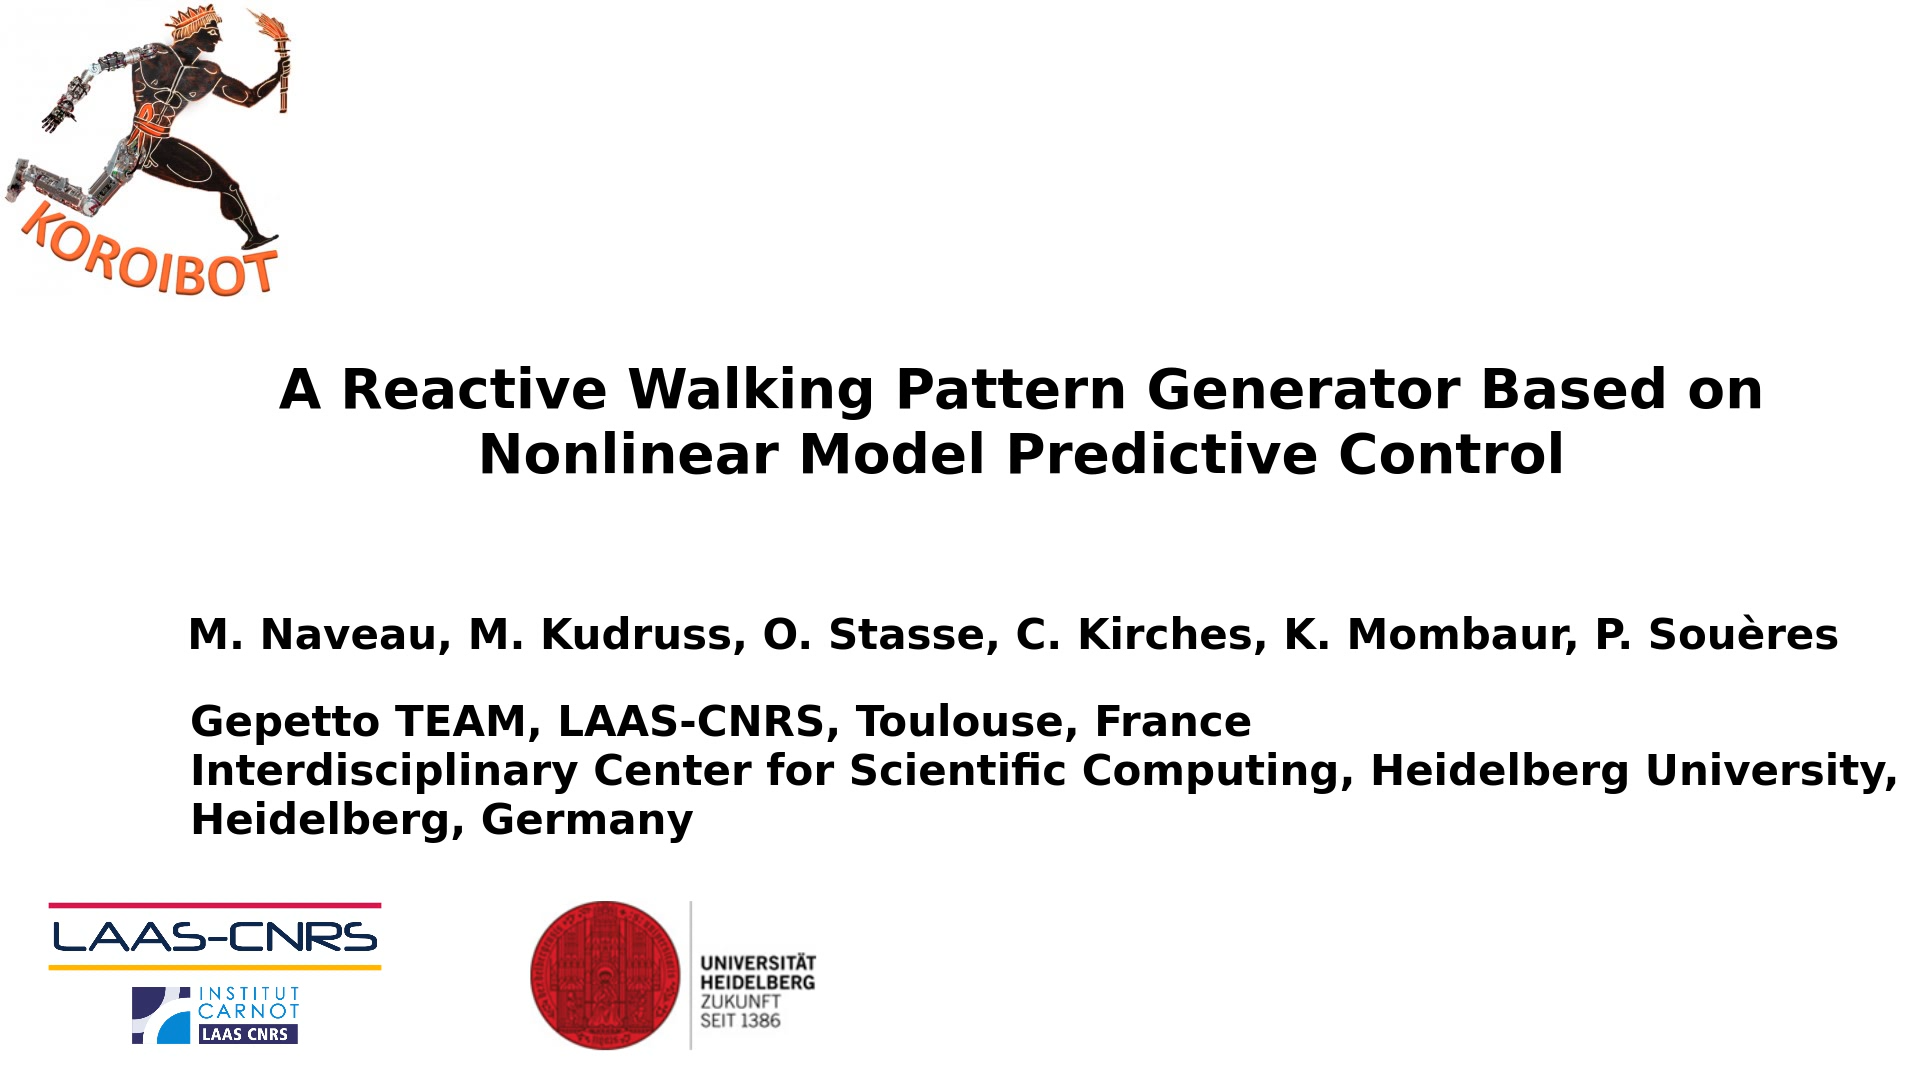
\includegraphics[width=0.85\linewidth, keepaspectratio]
      {16-raletter-NMPC-v19.png}    
    }  
    {videos/16-raletter-NMPC-v19.mp4}
  \end{center}
\end{frame}

%%%%%%%%%%%%%%%%%%%%%%%%%%%%%%%%%%%%%%%%%%%%%%%%%%%%%%%%%%%%%%%%%%%%%%%%%%%%%%%

